\chapter{Softwaredokumentation auf Github} \label{appendix:documentation}

 \iftoggle{isprint}{
Die Softwaredokumentation wurde in dieser Ausgabe der Arbeit ausgelassen und ist nur in der vollen, auf der CD ablegten Version oder auf \purl{https://www.github.com/upd89}, einzusehen.
}{

Auf den nachfolgenden Seiten ist die offizielle Dokumention von upd89 auf github.com abgebildet.

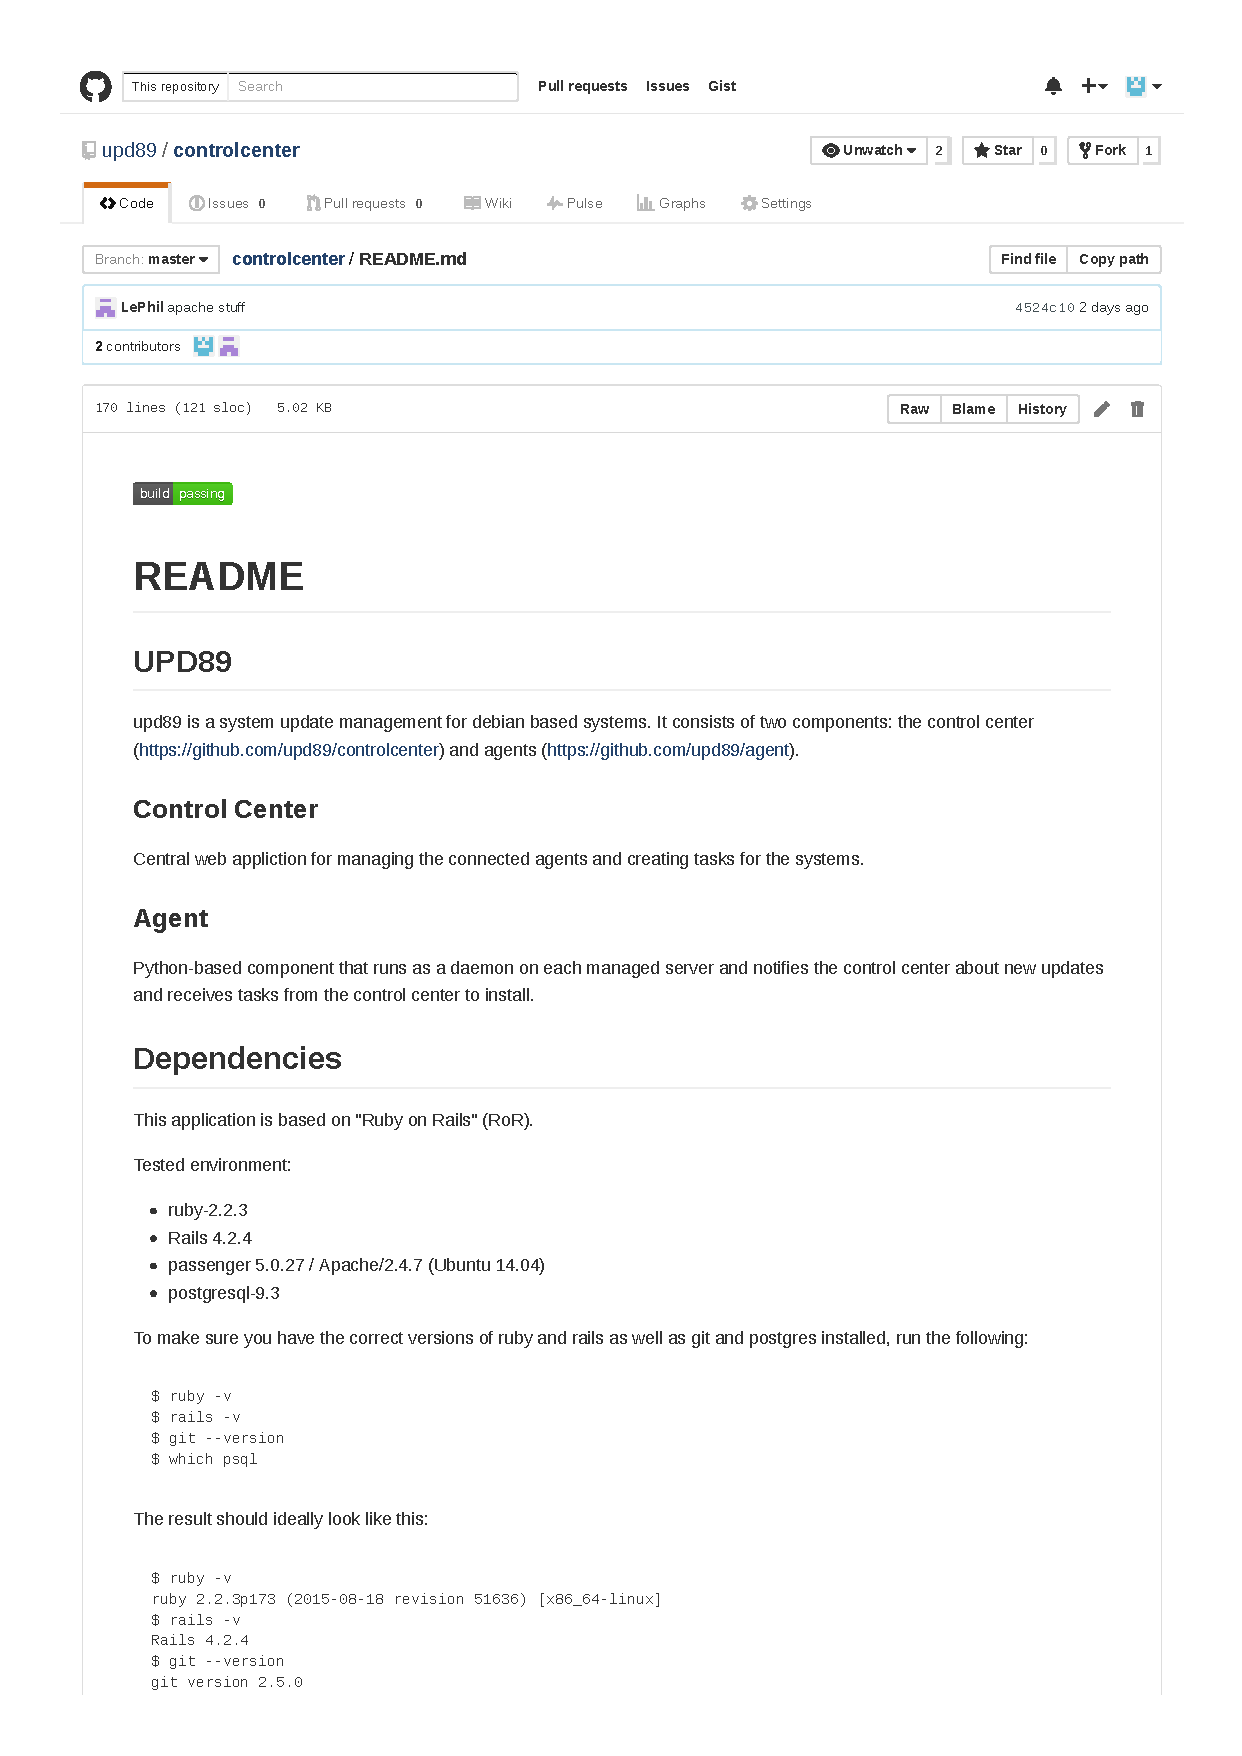
\includepdf[pages=1-,frame,scale=0.7,pagecommand={}]{fig/controlcenter_README}

%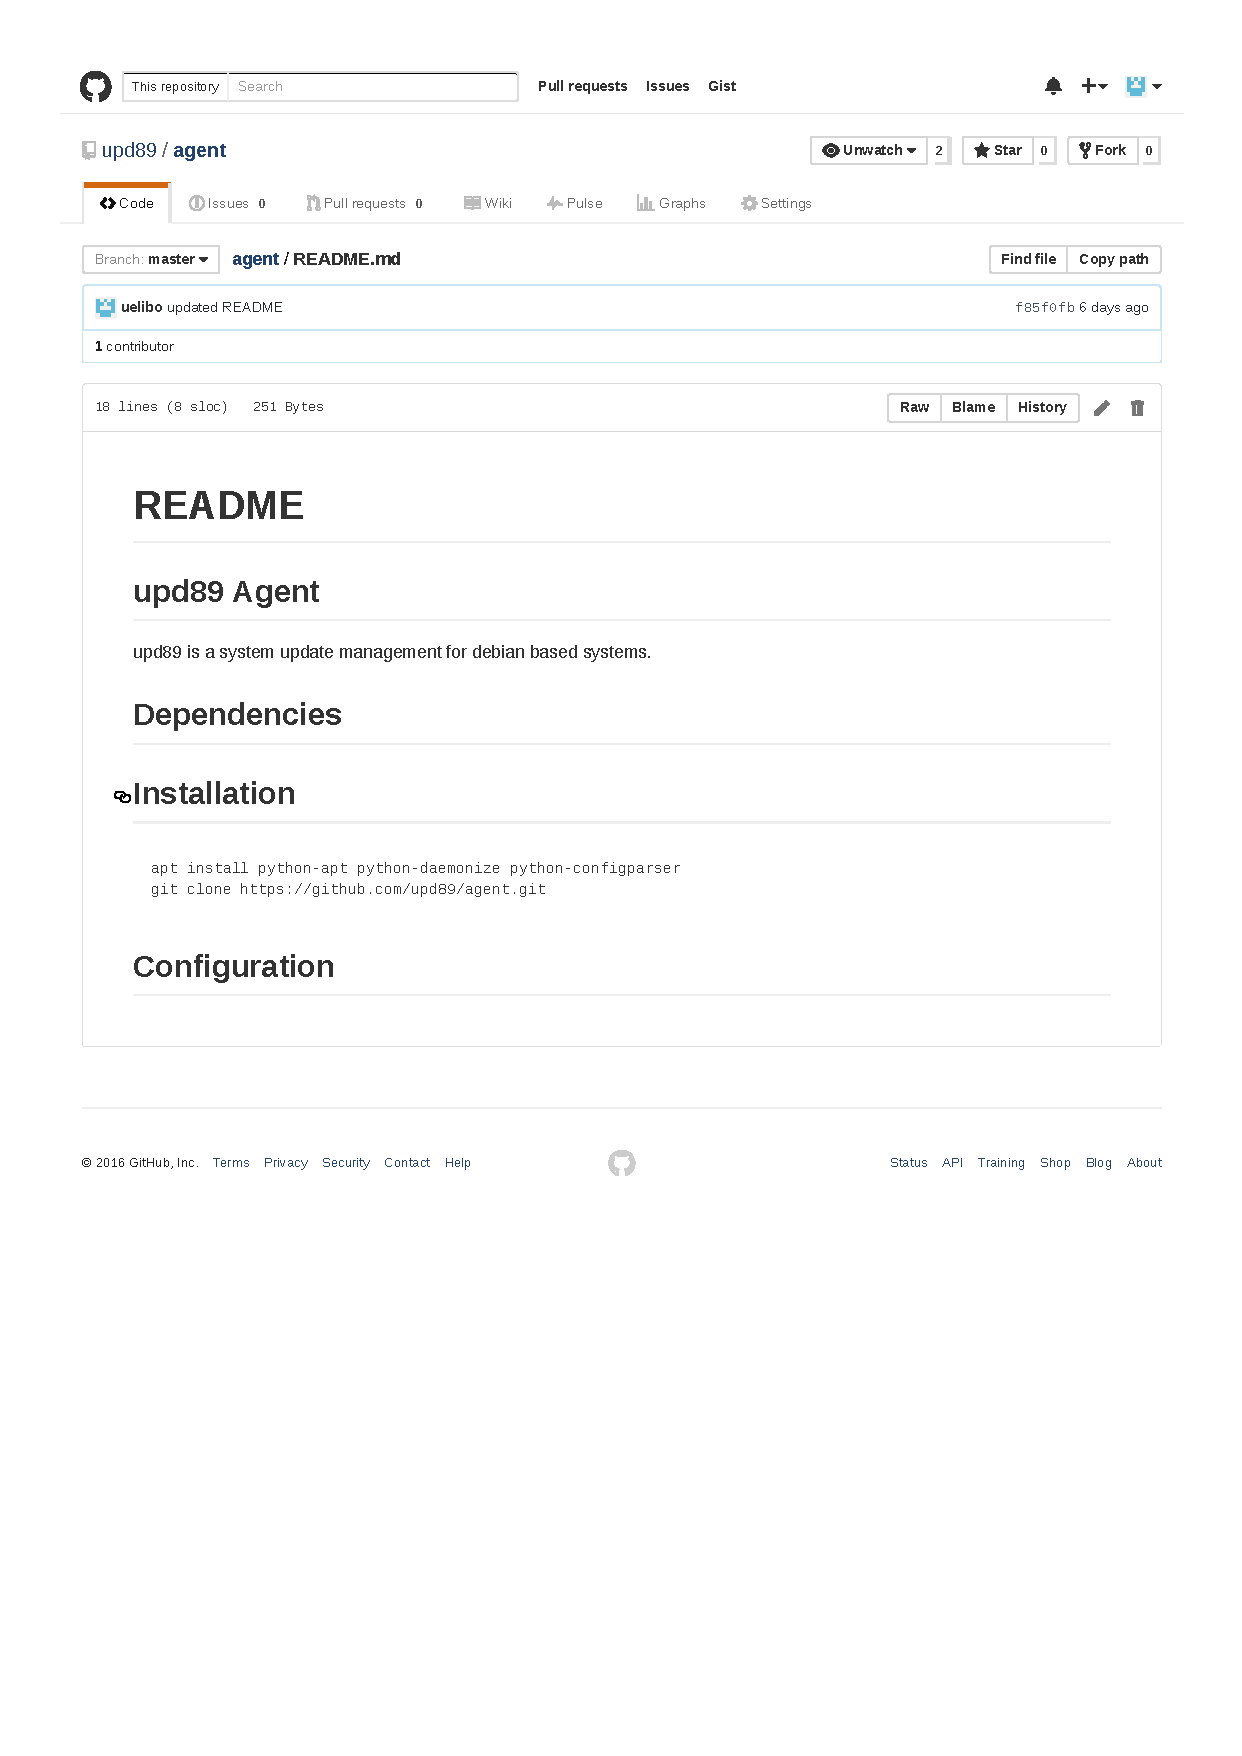
\includepdf[pages=1-,frame,scale=0.7,pagecommand={}]{fig/agent_README}

\begin{figure}
    \centering
    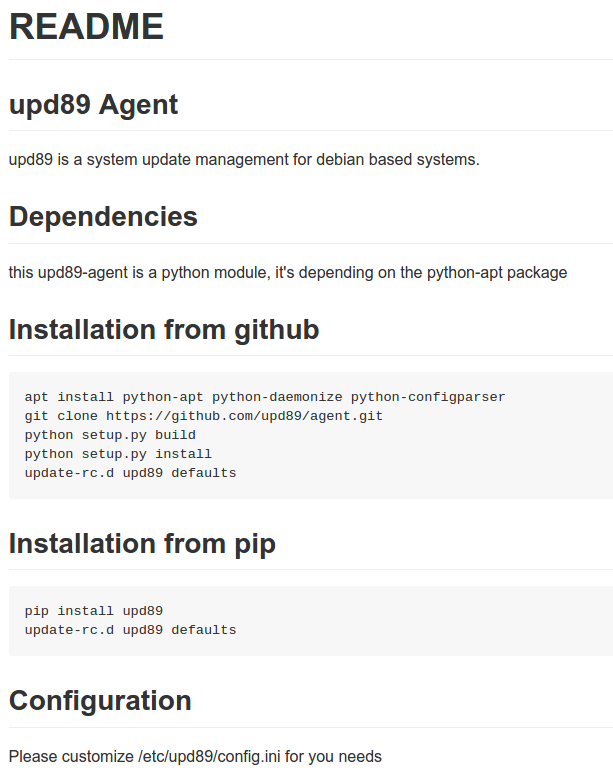
\includegraphics[width=0.8\textwidth]{fig/agent_readme}
    \caption{Readme des Agents}
    \label{fig:appendix:documentation:agent}
\end{figure}

}